\documentclass[final,table,14pt,aspectratio=141]{beamer}
\setbeamertemplate{navigation symbols}{}
\usepackage{graphicx}
\usepackage{tikz}
\usepackage{marvosym}
\usepackage{pgfpages}
\usepackage{hyperref}
\usepackage{fontawesome}
\urlstyle{rm}

%\usepackage{beamerposter}

\tikzstyle{na} = [baseline=-.5ex]
\usetikzlibrary{arrows,shapes,backgrounds}
\tikzstyle{every picture}+=[remember picture]
\usetikzlibrary{spy}


\usepackage{fontspec}
\defaultfontfeatures{Ligatures=TeX}
%\setmainfont[Path = /home/ctroupin/.fonts/]{Cube-Regular2}
\setmainfont{Droid Sans}
\setsansfont{Droid Sans}
%\setsansfont[Path = /home/ctroupin/.fonts/]{Cube-Regular2}
%\setromanfont[Path = /home/ctroupin/.fonts/]{DINM2}

\definecolor{bluegher}{RGB}{4,99,128}  		% blue 
\definecolor{greygher}{RGB}{50, 50, 50}  	% grey 
\definecolor{redgher}{RGB}{189, 33, 5}  	% red 
\definecolor{greybackground}{RGB}{235, 235, 235}

\hypersetup{colorlinks,linkcolor=,urlcolor=bluegher}

\setbeamerfont{title}{size=\scriptsize}
\setbeamerfont{subtitle}{size=\normalsize}
\setbeamerfont{date}{size=\scriptsize}
\setbeamercolor{title}{fg=bluegher}
\setbeamercolor{subtitle}{bg=bluegher,fg=white}

\setbeamersize{text margin left=1cm, text margin right=1cm} %new code

\defbeamertemplate*{title page}{customized}[1][]
{
  \usebeamerfont{title}\inserttitle\par
  \usebeamerfont{subtitle}\usebeamercolor[fg]{subtitle}\usebeamercolor[bg]{subtitle}\insertsubtitle
}
   
% ------------------------------------------------
% LENGTH DEFINITIONS
%-------------------------------------------------
%\setlength{\textwidth}{24cm}
%\setlength{\textheight}{28cm}
\setbeamersize{text margin left=10pt,text margin right=10pt}

\newcommand{\seplogo}{\hspace{.35cm}}
\newcommand{\figheight}{.05\textheight}
\newcommand{\putlogo}[1]{\includegraphics[height=\figheight]{#1}}
\newcommand{\putlogoB}[1]{\includegraphics[height=1.25cm]{#1}}

\DeclareGraphicsExtensions{.eps,.JPG,.jpg,.pdf,.png,.PNG,.jpeg}
\graphicspath{
{./logos/},
}

\parindent 0cm

\usebackgroundtemplate{\tikz\node[opacity=0.2]{\parbox[c][\paperheight][c]{\paperwidth}{\hspace{-.25cm}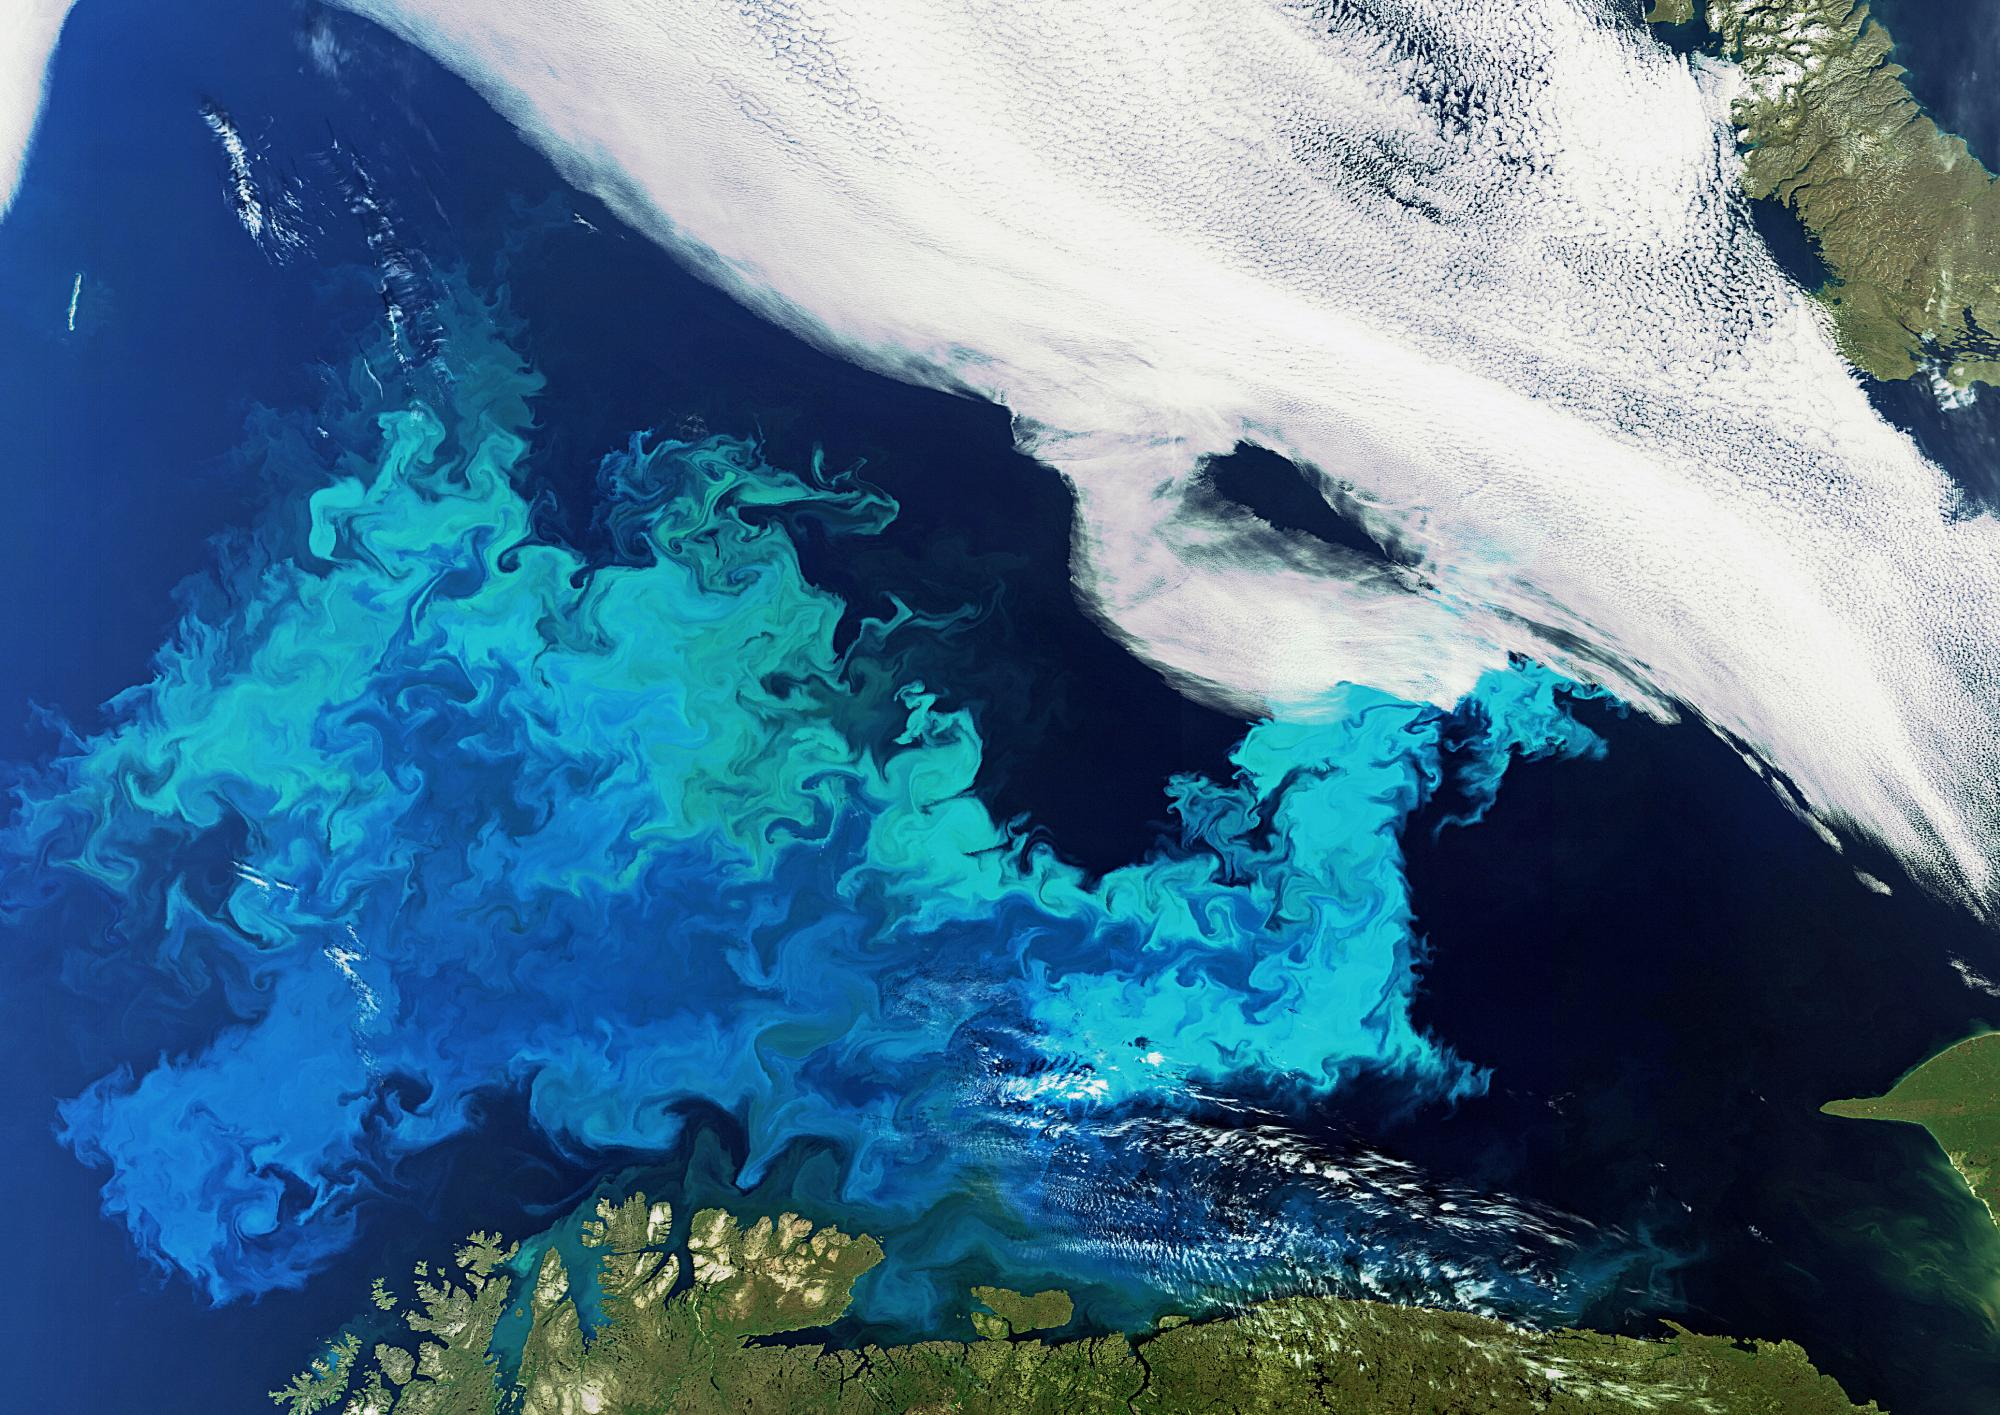
\includegraphics[width=1.05\paperwidth]{./background.jpg}}};}

\addtobeamertemplate{background}{}{%
\begin{tikzpicture}[remember picture,overlay]
\node[anchor=north east,yshift=-10pt,xshift=-.5cm] at (current page.north east) {
\includegraphics[height=.07\textheight]{logo_colloquium}};
\node[anchor=north west,yshift=-8.95cm,xshift=.25cm] at (current page.north west) {\tiny Image credit: ESA};


\end{tikzpicture}}

% These lines to keep good colors when viewed with Acrobat Reader
\makeatletter%
\special{pdf: put @thispage <</Group << /S /Transparency /I true /CS /DeviceRGB>> >>}%
\makeatother%

\author{}
%\url{www.socib.es}}
\title[]{48th International Liege Colloquium on Ocean Dynamics}
\subtitle{Submesoscale Processes:\\ Mechanisms, Implications and new Frontiers}
\date{23-27 May 2016}

\begin{document}

\begin{frame}[fragile]


\centering
\maketitle

\begin{tikzpicture}[remember picture,overlay]%
 
\coordinate (tp1) at ([yshift=-.25cm]current page.north west);
\coordinate (tp2) at ([yshift=-1.85cm]current page.north west);
\coordinate (tp3) at ([yshift=-1.85cm]current page.north east);
\coordinate (tp4) at ([yshift=-.25cm]current page.north east);

\coordinate (tp5) at (current page.south west);
\coordinate (tp6) at ([yshift=1.15cm]current page.south west);
\coordinate (tp7) at ([yshift=1.15cm]current page.south east);
\coordinate (tp8) at (current page.south east);
\filldraw[draw=none,fill=white,opacity=0.35] (tp1)--(tp2)--(tp3)--(tp4)--cycle;
\filldraw[draw=greygher,fill=white,opacity=0.6] (tp5)--(tp6)--(tp7)--(tp8)--cycle;
\end{tikzpicture}

%\vspace*{-.35cm}

\begin{columns}[totalwidth=1.\textwidth,c]

\column{.5\textwidth}

\begin{tikzpicture}[spy using outlines={circle,greygher,magnification=5,size=1.5cm, connect spies}]
\node[anchor=south west,inner sep=0] (image) at (0,0) {\pgfimage[interpolate=true,width=.6\textwidth]{main_fig2_resize.png}};
   
    \begin{scope}[x={(image.south east)},y={(image.north west)}]
%    \draw[help lines,xstep=.1,ystep=.1] (0,0) grid (1.2,1.2);
%    \foreach \x in {0,1,...,12} { \node [anchor=north] at (\x/10,0) {0.\x}; }
%    \foreach \y in {0,1,...,12} { \node [anchor=east] at (0,\y/10) {0.\y}; }
    \coordinate (pos spy) at (1.25,.9);
    \coordinate (center) at (.5,.85);
    \coordinate (pos spy2) at (1.8,.6);
    \coordinate (center2) at (.5,.6);
    \coordinate (pos spy3) at (1.35,.3);
    \coordinate (center3) at (.6,.25);
    
    \spy on (center) in node [] at (pos spy);
    \spy on (center2) in node [] at (pos spy2);
    \spy on (center3) in node [] at (pos spy3);
    
   	\path (1.25,.9) coordinate (ABC1);
	\path (1.8,.6) coordinate (DEFG1);
	\path (1.35,.3) coordinate (HIJ1);
   
    \end{scope}  
   
\end{tikzpicture}

\column{.25\textwidth}
\tiny
\tikz[na, xshift=-1cm] \coordinate (A0); Observations - Modelling - Theory\\
\tikz[na] \coordinate (A2); Air-sea coupling\\
\tikz[na, xshift=-1cm, yshift=-1ex] \coordinate (ABC2);\tikz[na] \coordinate (B2); Surface forcing \\
\tikz[na] \coordinate (C2); Remote-sensing \\
\tikz[na] \coordinate (D2); Fronts  \\
\tikz[na, xshift=-1cm, yshift=-1ex] \coordinate (DEFG2);\tikz[na] \coordinate (E2); Instabilities \\
\tikz[na] \coordinate (F2); Energy cascade \\
\tikz[na] \coordinate (G2); Turbulence \\
\tikz[na] \coordinate (H2); Coastal dynamics\\
\tikz[na, xshift=-1cm, yshift=-1ex] \coordinate (HIJ2);\tikz[na] \coordinate (I2); Freshwater\\
\tikz[na] \coordinate (J2); Waves\\
\tikz[na] \coordinate (K2); Biological interactions 

\begin{tikzpicture}[overlay]
\path[o-,greygher,thin] (ABC1) edge [out=0, in=180] (ABC2);
\path[-o,greygher,thin] (ABC2) edge [out=0, in=180] (A2);
\path[-o,greygher,thin] (ABC2) edge [out=0, in=180] (B2);
\path[-o,greygher,thin] (ABC2) edge [out=0, in=180] (C2);

\path[o-,greygher,thin] (DEFG1) edge [out=0, in=180] (DEFG2);
\path[-o,greygher,thin] (DEFG2) edge [out=0, in=180] (D2);
\path[-o,greygher,thin] (DEFG2) edge [out=0, in=180] (E2);
\path[-o,greygher,thin] (DEFG2) edge [out=0, in=180] (F2);
\path[-o,greygher,thin] (DEFG2) edge [out=0, in=180] (G2);


\path[o-,greygher,thin] (HIJ1) edge [out=0, in=180] (HIJ2);
\path[-o,greygher,thin] (HIJ2) edge [out=0, in=180] (H2);
\path[-o,greygher,thin] (HIJ2) edge [out=0, in=180] (I2);
\path[-o,greygher,thin] (HIJ2) edge [out=0, in=180] (J2);
\path[-o,greygher,thin] (HIJ2) edge [out=0, in=180] (K2);
\end{tikzpicture}

\end{columns}


\vspace{-0.02\textheight}
{ \rmfamily \tiny
\textcolor{greygher}{\faCalendarCheckO~~~\insertdate}\\
\textcolor{bluegher}{{\ComputerMouse}~~~\url{http://modb.oce.ulg.ac.be/colloquium}}\\
\textcolor{greygher}{\faHome~~~University of Liège - Place du 20-Août, 7 - 4000 Liège - Belgium}\\ 
\textcolor{bluegher}{\Letter}~~~\href{mailto:oceanphys@ulg.ac.be}{oceanphys@ulg.ac.be}\\
\textcolor{greygher}{\faTwitter~~~@GHER\_ULg}\\
}

\vspace{.05cm}
{\scriptsize 
\fcolorbox{black}{redgher}{\textcolor{white}{Deadline for abstract submission: 30th January 2016}}
}

{\scriptsize 
\href{http://modb.oce.ulg.ac.be/colloquium/2016/#col_travel_grants}{Travel support}: please visit the colloquium web page
}

\vfill
%\vspace*{-.25cm}

\begin{columns}[totalwidth=1.\textwidth,c]

\column{.2\textwidth}
\scriptsize
%\textcolor{black}{Organised by}

%\vspace{.1cm}

\putlogo{logo_gher}\seplogo\putlogo{logo_imedea}\seplogo\putlogo{logo_whoi} %\seplogo\putlogo{logo_ulg}\\

\column{.05\textwidth}
~
\column{.75\textwidth}

\scriptsize
%with the support of\\
\putlogo{coq_wallon}\seplogo\putlogo{logo_IOC}\seplogo\putlogo{logoSocib}\seplogo\putlogo{logo_CNES}\seplogo\putlogo{logo_esa}\seplogo \putlogo{logo_nasa}\seplogo\putlogo{logo_onr}\seplogo\putlogo{logo_iugg}%\putlogoB{logo_egu}%\seplogo\putlogo{logo_SCOR}\seplogo

\end{columns}

\end{frame}



\end{document}
